\documentclass{article}

% set font encoding for PDFLaTeX or XeLaTeX
\usepackage{ifxetex}
\ifxetex
  \usepackage{fontspec}
\else
  \usepackage[T1]{fontenc}
  \usepackage[utf8]{inputenc}
  \usepackage{lmodern}
\fi
\usepackage{graphicx}

% used in maketitle
\title{Actividad 2}
\author{Roberto Alexis Gómez Pintor}


% Enable SageTeX to run SageMath code right inside this LaTeX file.
% documentation: http://mirrors.ctan.org/macros/latex/contrib/sagetex/sagetexpackage.pdf
% \usepackage{sagetex}

\begin{document}
\maketitle
\section{Reporte}
\subsection{Introduccion}
Usa un sistema basado en Kernel. Cada Kernel es un motor de ejecución para un lenguaje o plataforma concreta que ejecuta en el servidor. Podemos ejecutar Jupyter localmente en nuestro sistema. Instalarlo es tan fácil como instalar Anaconda, la plataforma abierta para data science basada en Python, o directamente con la herramienta de instalación de paquetes de Python. Jupyter es una herramienta libre fantástica que se está convirtiendo en el standard en el mundo del análisis de datos. La comunidad que lo impulsa es muy activa y heterogénea, lo que está enriqueciendo el desarrollo y la integración con otras herramientas y plataformas. Las graficas estan basadas en datos de la region Cumbres Monterrey, Nuevo Leon, México.
\begin{figure}
  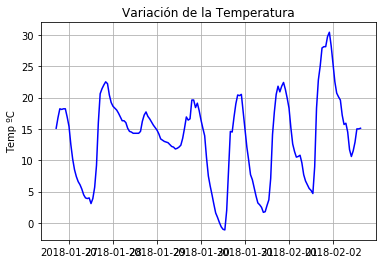
\includegraphics[width=\linewidth]{temperatura.png}
  \caption{Varianza de la temperatura.}
  \label{fig:boat1}
\end{figure}

\begin{figure}
  \includegraphics[width=\linewidth]{temperaturahumedadrelativa.png}
  \caption{Variacion de temepratura y humedad relativa.}
  \label{fig:boat1}
\end{figure}

\begin{figure}
  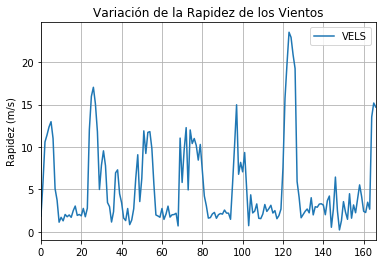
\includegraphics[width=\linewidth]{vels.png}
  \caption{A boat.}
  \label{fig:boat1}
\end{figure}

\subsection{Preguntas}
\subsubsection{¿Cuál es tu primera impresión de Jupyter Notebook?}
Un sitio web para el manejo de datos, desarrollo de los lenguajes de programacion de forma abierta y gratuita permitiendo al usuario trabajar.
\subsubsection{¿Se te dificultó leer código en Python?}
Un poco para entender, aunque la mayor parte del trabajo fue realizada por el mismo sitio web, permitiendo una flexibilidad al entender.
\subsubsection{¿En base a tu experiencia de programación en Fortran, que te parece el entorno de trabajar en Python?}
Creo que a diferencia del lenguaje de programacion FORTRAN no tuve tanto trabajo para realizar las actividades nencesarias,debido a que permetia hacer las cosas sin necesariamente aprender sobre las herramientas.
\subsubsection{A diferencia de Fortran, ahora se producen las gráficas utilizando la biblioteca Matplotlib. ¿Cómo fue tu experiencia?.}
Bastante comodo, no tenia que preocuparme de si alguno dato estuviera mal no fuera graficado, simplemente me mostraba el dato donde estaba y asi viendo la grafica podia ver en que parte estaba mal y no tener que rehacer todo el codigo.
\subsubsection{En general, ¿qué te pereció el entorno de trabajo en Python?}
Me parecio un ambiente comodo de trabajo sin tener que construir tanto codigo como en Fortran.
\subsubsection{¿Qué opinas de la actividad? ¿Estuvo compleja? ¿Mucho material nuevo? ¿Que le faltó o que le sobró? ¿Qué modificarías para mejorar?}
Lo complciado en la actividad fue que al elejir yo la ciudad tenia una extension de datos mas de lo normal, la dificultad en general seria tipo medio, no era muy facil ni dificil, no encuentro algo que deba modificar.
\subsubsection{¿Comentarios adicionales que desees compartir?}
Ningun comentario
\end{document}
